\documentclass[10pt,oneside]{book}

% Margenes
\usepackage[left=3cm,top=3cm,right=3cm,bottom=3cm]{geometry} %%Márgenes

% Paquetes a usar
\usepackage[spanish,es-lcroman,activeacute] {babel}   %%para Colocar el Español
\usepackage[utf8]{inputenc}
\usepackage{amsmath}          % Ecuaciones
\usepackage{amssymb}          % Símbolos 
\usepackage{graphicx}         % Graficos
\usepackage{graphics}         % Subfiguras
\usepackage{pdfpages}         % incluir PDF
%\usepackage[tight,footnotesize]{subfigure}
\usepackage{parskip}
\usepackage[pdftex, plainpages=false, hypertexnames=false, pdfpagelabels=true,
    hyperindex=true, linktocpage, pagebackref=true, pdfa=true]{hyperref}         % Vinculos
\usepackage{color}
\usepackage{float}					 %Fijar figuras a gusto
\usepackage{array}
\usepackage{caption}
\usepackage{subcaption}
\usepackage{titlesec} 				%Cambio de estilo de títulos
\usepackage[titletoc,title]{appendix}
\usepackage{mathrsfs}


% Cambiar nombre de elmentos 
\renewcommand{\partname}{Parte}
\renewcommand{\chaptername}{Capítulo}
\renewcommand{\appendixname}{Apéndice}
\renewcommand{\bibname}{Referencias}
\renewcommand{\figurename}{Figura}
\renewcommand{\spanishtablename}{Tabla}
\renewcommand{\labelitemi}{$\bullet$}
\renewcommand{\arraystretch}{1.6}

\setlength{\parskip}{3.1mm plus2mm minus2mm}
\let\cleardoublepage\clearpage %Quitar paginas en blanco
\setlength{\parindent}{0pt} % Quitar sangria del inici de parrafo

%Cambio del estilo para los títulos de los chapters
\titleformat{\chapter}
  {\normalfont\Huge\bfseries}{\thechapter.}{1em}{}

% Inicio del documento
\begin{document}

%Eliminar bordes rojos de los hipervinculos
\hypersetup{pdfborder=0 0 0}

% Porta del documento
\thispagestyle{empty}

% Numero de tesis
%\underline{N$ ^\circ  $ tesis:} jcb

\begin{center}

\vspace{2.5cm}

\begin{large}
\textbf{PROYECTO FIN DE CARRERA}\\

\vspace{0.7cm}

Presentado a\\

\vspace{0.7cm}

\textbf{LA UNIVERSIDAD DE LOS ANDES\\
FACULTAD DE CIENCIAS\\
DEPARTAMENTO DE FÍSICA}\\

\vspace{1.5cm}

Para obtener el título de\\

\vspace{0.7cm}

\textbf{FISICO}\\

\vspace{1cm}

por\\ 

\vspace{0.7cm}

\textit{\textbf{Camilo Andrés Rivera Lozano}}\\

\vspace{1cm}

\rule[10pt]{\textwidth}{1pt}
\textbf{\textit{IMPACTO DE LOS PARÁMETROS COSMOLÓGICOS EN LA ESTRUCTURA A GRAN ESCALA DEL UNIVERSO}}\\
\vspace{0.7cm}
\rule[10pt]{\textwidth}{1pt}

\vspace{1cm}

Sustentado el -- de Diciembre de 2014 frente al jurado:

\vspace{1cm}

\textbf{\underline{Composición del jurado}}

\vspace{1cm}

\end{large}

\begin{tabular}{p{0.02\textwidth}p{0.1\textwidth}p{0.8\textwidth}}
-	&	\textit{Asesor:}	&  Jaime E. Forero-Romero PhD, Profesor Asociado, Universidad de Los Andes\\
\end{tabular}

\end{center}



% Dedicatoria
\newpage

% Pagina sin numeración
\thispagestyle{empty}
\begin{tiny}

\end{tiny}

\vspace{5cm}

\begin{flushright}
\begin{large}
\textit{punto.}\\
\hfill
\textit{A todos, gracias...}
\end{large}
\end{flushright}

% Agradecimientos
% Pagina sin numeración
\thispagestyle{empty}

\chapter*{Agradecimientos}



% Colocar numeración romana para tabla de contenido
\setcounter{page}{1}
\pagenumbering{roman}


%Tabla de contenidos
\renewcommand{\contentsname}{Tabla de contenido}
\tableofcontents
%Tabla de Figuras
\renewcommand{\listfigurename}{Índice de figuras}
\listoffigures 
%Tabla de Tablas
\renewcommand{\listtablename}{Índice de tablas}
\listoftables

% Colocar numeración Arabica para el resto del contenido
\newpage
\setcounter{page}{1}
\pagenumbering{arabic}


% Introducción
\chapter{Introducción}

El universo, su composición y evolución han sido objeto de estudio para el hombre desde tiempos incluso anteriores a poseer la capacidad para ver más allá del cielo. La innegable inmensidad del universo nos deja sin más remedio que la observación para su caracterización y, siendo lo más rápido del universo, la luz es por excelencia el método a través del cual podemos ahondar en los secretos que esconde.

El creciente desarrollo de la tecnología, la mejora en la sensibilidad de los equipos y la capacidad de computación para el análisis de los datos nos han brindado un mejor panorama de cómo es el universo, tanto local como a gran escala, pero el hecho que finalmente nos mostró la verdad sobre la historia y antigüedad del universo fue el descubrimiento y análisis del fondo de radiación de microondas. No sólo fue el sustento para la teoría del \textit{Big-Bang} sino que también nos mostró como fue el universo en momentos cercanos a su origen, justo después de la recombinación cuando el universo se volvió transparente y la luz pudo finalmente viajar libremente. 

Estos análisis nos permitieron conocer a fondo la composición del universo y caracterizarlo a partir de los que hoy se conocen como los parámetros cosmológicos, pero ¿qué tan diferente sería el universo si variaran dichos parámetros? Lamentablemente contamos con un único universo y el método de la experimentación es inviable pues las condiciones en las que se generó el universo exceden por mucho nuestras capacidades, de manera que la única alternativa para responder esta pregunta yace en las simulaciones computacionales a gran escala. 

La creación de máquinas de muy alto nivel de procesamiento y la paralelización de tareas a lo largo de un gran número de procesadores ($>50$) ha permitido la creación de simulaciones cada vez más grandes en un lapso de tiempo cada vez menor. Las simulaciones de N cuerpos permiten observar la evolución del universo y extraer información de las posibles diferencias en cada uno de los escenarios propuestos. En la actualidad se encuentran en desarrollo diferentes experimentos, entre otros el DESI\cite{desi} y el HETDEX\cite{hetdex}, que pretenden medir y cuantificar los efectos de la energía oscura en el universo, de manera que los resultados de este proyecto podrán contrastarse con los datos arrojados por estos experimentos mostrando la distribución de energía-materia que más se acopla a nuestro universo.

El siguiente documento presenta la planeación, desarrollo y resultados de un trabajo que consistió en la generación de condiciones iniciales para universos con diferentes parámetros cosmológicos, la simulación en paralelo de la evolución de dichos universos y el análisis de los estados finales de cada simulación. Para esto se hizo uso de la paralelización del trabajo en cajas con condiciones periódicas de entre 150Mpc y 500Mpc, un número de partículas entre $128^3$ y $512^3$ y un tiempo de simulación cercano a los 13Gyr. El análisis realizado a cada estado final fue hecho a través del lenguaje C, mientras que la visualización de los datos fue realizada a través de Python. 

En el Capítulo \ref{chap:marco} se explicarán las bases teóricas y los conocimientos pertinentes que fueron requeridos para el desarrollo del proyecto, desde el funcionamiento de una simulación en paralelo, la historia del universo y la descripción de los parámetros cosmológicos. Posteriormente en el Capítulo \ref{chap:metodologia} se explicará brevemente la metodología planteada y usada a través del desarrollo del proyecto, el plan de trabajo y los pasos que se siguieron. Luego, en el Capítulo \ref{chap:trabajo}, se mostrarán los resultados del trabajo realizado, así como los problemas encontrados, los códigos y programas creados y la intercomunicación entre estos.

\section{Motivación}
Las mediciones más recientes de las anisotropías del universo primitivo, grabadas en el CMB, fueron realizadas por la sonda Plank en donde se establecieron los valores más actualizados de los parámetros cosmológicos. De todas maneras, aún quedan muchas incógnitas por resolver, y son grandes cambios los que se pueden alojar dentro del margen de error de las mediciones. Este proyecto trabaja desde el marco de las simulaciones, realizando variaciones del $5\%$ en la densidad de materia en el universo alrededor de las mediciones de la sonda Plank, para identificar los rasgos que caracterizan dichas variaciones. En especial se centra en las diferencias observables de la formación y dinámica de los halos de materia oscura, como lo son sus velocidades de centro de masa y su abundancia en el universo. Estos datos enriquecerán los datos de las mediciones y correcciones realizadas sobre los parámetros cosmológicos, permitiendo un análisis más profundo en donde se puede correlacionar las mediciones con las observaciones de efectos indirectos.


\section{Objetivos}

\subsection*{General}
Cuantificar el cambio de la estructura a gran escala del universo ante escenarios con diferentes parámetros cosmológicos.
\subsection*{Específicos}
\begin{itemize}
	\item Obtener una serie de universos simulados ante diferentes valores de parámetros cosmológicos.
	\item Extraer información acerca de los diferentes universos como la abundancia de halos de materia oscura y las distribuciones de velocidad entre pares de halos.
	\item Realizar un análisis comparativo entre los diferentes universos simulados
\end{itemize}

%Marcos
	\chapter[Marco Teórico]{Marco Teórico}
\label{chap:marco}
\section{La evolución del universo}
\label{sec:universo}
El universo tal y como lo conocemos hoy está poblado de cuerpos colosales, sorprendentes e incluso hermosos. Las estrellas, las nébulas y las galaxias son formaciones a las que estamos acostumbrados y que están presentes en donde quiera que nos adentremos en el cielo. Pero fue un proceso muy largo y turbulento para llegar a lo que hoy observamos y consideramos habitual, como nuestro sistema solar, un proceso que aún está lleno de incógnitas y de teorías que si bien se ajustan a las observaciones y predicciones, no están completamente comprobadas. La siguiente sección trata de resumir el conjunto de teorías y hechos que hacen parte de la visión más ampliamente aceptada como la historia del universo.


\subsection{El Principio cosmológico y el problema del Horizonte}
Las teorías que describen los momentos que precedieron al \textit{Big-Bang} y el análisis del fondo de radiación de microondas (CMB por sus siglas en inglés) han brindado un panorama de lo que que parece ser el inicio del universo y su progreso hasta lo que conocemos hoy en día; un universo que cumple con el principio cosmológico\cite{loeb}. Las fórmulas de la relatividad general de Einstein muestran cómo la estructura del Espacio-Tiempo se ve curvada por la presencia de la masa, pero al intentar aplicar estas fórmulas para mostrar la dinámica del universo, hay que considerar un modelo para éste. Dada la complejidad matemática que pueden llegar a tener estas fórmulas en el caso general, fue necesario considerar el caso más simple posible, dictado por el principio cosmológico. Bajo este principio, el universo es isotrópico y homogéneo, lo cual quiere decir que el universo tiene una distribución homogénea y esta distribución se cumple en cualquier dirección en la cual se observe. Se podría pensar que los planetas, estrellas, galaxias y otros cuerpos nombrados anteriormente, los cuales además de todo están separados por vastos vacíos casi absolutos, serían el perfecto contraejemplo para la suposición de Einstein, pero este enunciado hace referencias a escalas mucho mayores a las que podría abarcar cualquiera de estos cuerpos. Para dar una idea de la escala de distancias tratadas, la Vía Láctea tiene un tamaño aproximado de $30kpc$, pero si partimos el universo en cubos, por ejemplo de $90Mpc$, veremos que estos cubos comparten características casi idénticas, como por ejemplo, la densidad promedio, emisión de luz e incluso temperatura \cite{bang}. 

Este hecho antes de ser tranquilizante (vivimos en lo que sería el caso ideal de un universo), es bastante alarmante puesto que no puede ser coincidencia que lugares tan apartados del universo posean la misma temperatura, y no son dos lugares sino todos los rincones observados del universo los que cumplen con dicho principio. El problema radica en que la forma de comunicación más rápida existente entre dos cuerpos es la luz, y por ende la \textcolor{red}{comunicación} entre dos lugares del universo estará limitada por la distancia que los separa. De esta manera, si consideramos que el universo tiene una edad aproximada de $13.8Gyr$, no hay forma para que dos puntos opuestos (separados por $\approx 28Gly$) hayan tenido algún intercambio tal que les hubiese permitido estar en condiciones iguales hoy en día. 


\subsection{La Era Inflacionaria}
\label{sub:infl}
La teoría que hasta la fecha mejor resuelve esta incongruencia conocida como el \textit{Problema del Horizonte} es la teoría de la inflación. Ésta supone que en sus primeros instantes (al rededor de tiempos de $\sim 10^{-33} seg$), el universo pasó por un proceso de crecimiento acelerado, llegando incluso a velocidades superlumínicas. Existen varias versiones de esta época y no se ha logrado explicar a fondo la física detrás de este comportamiento. Entre las formas de explicarlo o describirlo, una explica que esta expansión se dio gracias a un estado que se conoce como \textit{falso vacío}, el cual no es mínimo estado de la densidad energética para un campo escalar, pero sí es un mínimo local, sólo que es inestable. En dicho estado se pudo dar una inflación de una sección tan pequeña que pudiese ser homogénea en sí, causando que el espacio resultante de la inflación replicara estas características. Dado el carácter atractivo (signo negativo) de la fuerza gravitacional es posible una expansión en donde se conserve la energía (Se ``crea'' energía al expandir que es compensada por la \textit{energía negativa} de la gravedad)\cite{bang}. 

\begin{figure}[H]
	\centering
	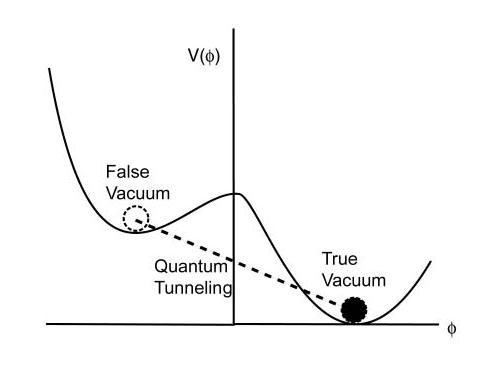
\includegraphics[width=8.5cm]{MarcoTeorico/figure7}
	\caption[Falso vacío y verdadero vacío ]{Falso vacío y verdadero vacío \footnotemark}
	\label{fig:falsevac}
\end{figure}
\footnotetext{Imagen tomada de \url{http://ned.ipac.caltech.edu/level5/Watson/Watson5_3.html}}

Otra forma de ver la inflación es pensando en que cualquier irregularidad presente en el universo cuando aún cabía en la palma de la mano se vería alisada por una expansión de dichas magnitudes. La difusión de los primeros fotones logró erradicar cualquier irregularidad en pequeña y gran escala de toda la materia ligada a la radiación electromagnética\cite{loeb}. En cualquiera de los casos, el resultado final de la inflación es un universo con las características que observamos en todas direcciones. 

Se cree que las galaxias y cuerpos que actualmente pueblan el universo se generaron a raíz  de las fluctuaciones cuánticas presentes en él cuando su tamaño fue lo suficientemente pequeño para que éstas tuvieran un efecto relevante en su estructura. En ese caso estas fluctuaciones de pequeña escala crecerían hasta tener un gran tamaño y se convertirían con el paso del tiempo en lo que hoy observamos como cuerpos estelares. Pero \textit{¿cómo es que estas fluctuaciones cuánticas siguieron presentes si la época inflacionaria borró cualquier irregularidad dando a un universo homogéneo?} La respuesta reside en cerca de un cuarto del contenido energético del universo: la materia oscura. 

\subsection{La inestabilidad gravitacional y la composición del universo}
\label{sub:grav}
Observaciones y mediciones de los espectros de galaxias y estrellas lejanas no sólo nos brindan información de su composición, sino que también de su dinámica. Las alteraciones en el espectro pueden deberse a varios factores, en especial el corrimiento hacia el rojo, para el cual existen tres principales motivos. El primero es debido al Efecto Doppler, que al igual que con el sonido, la longitud de onda aumenta (se corre hacia el rojo) cuando el emisor y el observador se alejan a grandes velocidades; el segundo es dictado por la relatividad general, cuando una onda electromagnética está escapando de un campo gravitacional; y el tercero, de mayor interés para efectos de la discusión a seguir, es el corrimiento al rojo (o \textit{redshift}) intrínseco debido a la expansión del universo. 

Observaciones de diferentes espectros atómicos en el universo han mostrado que incluso corrigiendo los corrimientos dados por movimientos relativos y por campos gravitacionales, siempre hay un corrimiento al rojo remanente. Un fotón emitido en un dicho momento tendrá una longitud de onda definida, pero si el universo se expande (el espacio donde se desplaza se expande), al cabo de un tiempo este fotón tendrá una longitud de onda menor que la que tenía inicialmente. De esta manera se ha observado que el universo se está expandiendo, y además es una herramienta de gran utilidad para definir distancias de objetos lejanos. Al observar objetos distantes, observamos su pasado, pues lo que nos llega es la luz emitida tiempo atrás, cuando el universo era un poco más pequeño, de manera que a mayor redshift en el espectro, más antiguo es el objeto que observamos.

Si consideramos que la densidad es constante en el universo, esto permite realizar un análisis local obviando el efecto del resto del universo dada la simetría esférica. La energía total por unidad de masa en una esfera de radio $r$ es una expresión dada por la suma de energía cinética, por el movimiento de las partículas, y la energía gravitacional potencial existente entre estas, así, $E=\frac{1}{2}v^2-\frac{GM}{r}$, en donde $G$ es la constante gravitacional y M estará dada considerando una densidad $\rho$ uniforme en el volumen de la esfera. Reorganizando los términos, se puede llegar a la Ecuación (\ref{eq:En}), en donde $\Omega=\frac{\rho}{\rho_c}$ y el término $\rho_c$ se conoce como la densidad crítica.

\begin{equation}
E=\frac{1}{2}v^2(1-\Omega)\\
\label{eq:En}
\end{equation}

Si la densidad promedio de materia en el universo $\rho$ es menor que la densidad crítica $\rho_c$  entonces tendremos que $E<0$ lo cual significa que la gravedad nunca podrá contrarrestar la expansión actual y toda galaxia está condenada a una muerte solitaria pues esta expansión continuará indefinidamente. Esto se conoce como la solución de un universo abierto. En cambio, si la densidad está por encima de la densidad crítica se tiene que la expansión se detendrá en un punto y comenzará a revertirse debido a la atracción gravitacional terminando en lo que se ha acuñado como el \textit{Big-Crunch}. Esta segunda solución se conoce como el universo cerrado. Finalmente, la tercera solución corresponde al universo plano en la que $E=0$ y la densidad de materia es exactamente igual a la densidad crítica. Esta tercera es la que se ha observado que coincide con la realidad, pero este es un equilibrio críticamente inestable, ya que por más homogéneo que se considere el universo, cualquier fluctuación crecerá con el paso del tiempo. Así si una pequeña sección supera la densidad crítica, comenzará a ejercer una mayor fuerza que el resto del universo, absorbiendo materia de las partes en donde la densidad es menor a la crítica. Rápidamente la parte densa se volverá más y más densa, contrario a lo que sucede con las secciones menos densas; una vez roto el equilibrio no hay vuelta atrás.

Como se dijo en la Sección \ref{sub:infl}, la inflación eliminó cualquier fluctuación de materia interactuante con la radiación, de manera que se estableció un equilibrio irrompible, en donde la formación de estrellas y galaxias se vuelve imposible. La materia oscura es la teoría de mayor acogida y validez para romper no sólo esta paradoja, sino que también otros fenómenos observados como las lentes gravitacionales y las velocidades de rotación de sistemas binarios. Para todos estos, se necesita que exista una cantidad de materia mayor que la observada; es decir, una cantidad mayor de materia que la que interactúa con la radiación electromagnética (materia ordinaria). De allí su nombre, la materia oscura es un tipo de materia con las mismas características gravitacionales que la materia ordinaria, pero no interactúa con ningún tipo de luz, de manera que no se puede observar de manera directa. La única forma de detectarla es por efectos indirectos, como la medición la cantidad de materia necesaria para que los fenómenos nombrados anteriormente tengan un sentido físico. 

Volviendo al universo primitivo, las fluctuaciones cuánticas generaron cambios en todo tipo de materia, pero la inflación sólo afecto aquella materia interactuante con la radiación, de manera que estas irregularidades quedaron grabadas en la materia oscura y crecieron junto con todo el universo. Esto creó regiones con mayor atracción gravitacional, causando que la materia ordinaria cayera en dichas zonas, juntándose, creciendo y formando cuerpos celestes. De manera que (bajo este punto de vista) es gracias a la presencia de la materia oscura que se pudo dar un universo tal y como lo conocemos, y es más, simulaciones de muy alto nivel de cuerpos de materia oscura, en comparación con las imágenes de estructura a gran escala del universo, muestran que la materia ordinaria se organiza exactamente en donde se generan mayores concentraciones de materia oscura, por el efecto nombrado anteriormente. Mediciones de la distribución de materia muestran que la materia oscura suma aproximadamente un $25\%$ de la energía total del universo, mientras que la materia ordinaria forma alrededor de un $5\%$. 

Estos porcentajes se conocen por mediciones y estimaciones, e incluyéndolos en la Ecuación (\ref{eq:En}), puesto que según las observaciones el universo debería ser plano y $\rho\approx\rho_c$. Al sumar toda la densidad de materia oscura y materia ordinaria, aún faltaría un gran porcentaje de densidad energética para cumplir la condición nombrada arriba, de manera que se plantea la energía oscura para cumplir con esa cuota. Es muy poco lo que se sabe acerca de la energía oscura y son muchas las teorías y vertientes entorno a ella, desde la energía de polarización de vacío hasta un fluido que llena todo el espacio tiempo. Entre las cosas que se pueden afirmar de ésta es que es cerca del $70\%$ del contenido energético del universo y es la responsable de la expansión de este (contrarrestada únicamente por la materia que conforma el otro $30\%$).


\subsection{Variables Relevantes y Parametrizaciones} 
Una vez explicada la historia que conllevó a la evolución del universo, es importante rescatar las parametrizaciones de cada fenómeno nombrado anteriormente, puesto que estas variables son los parámetros de ingreso a las simulaciones que se realizaron. Empezando por la expansión del universo, esta se mide por un factor de escala $a(t)$ que varía con el tiempo, tiene un valor de $1$ en la actualidad y para su definición se dice que si una distancia tiene una longitud $r(t_1)$ en dicho tiempo, entonces en $t_2$ estará definido por,

\begin{equation}
r(t_2)=r(t_1)\left[\frac{a(t_2)}{a(t_1)}\right]
\label{eq:at}
\end{equation}

Este factor es el que permite llevar cuenta de la expansión del universo a lo largo de una simulación, y puede definirse a partir del \textit{redshift} $z$, $a(t)=\frac{1}{1+z(t)}$ del cual se hablaba en la Sección \ref{sub:grav}. En la Figura \ref{fig:red} se observa un diagrama que muestra la historia del universo desde el Big-Bang, en la parte más externa cuando $z$ tiende a infinito, hasta la actualidad en el centro, donde $z=0$. Bajo este parámetro se fijan los tiempos de simulación y los intervalos de generación de \textit{snapshots} para las simulaciones realizadas. Asimismo, debemos incluir la versión matemática de la ley de expansión de Hubble, en donde se establece (a partir de observaciones) que la velocidad relativa (y por ende el corrimiento al rojo) de un objeto distante será proporcional a su distancia, donde $H_0$ es conocida como la constante de Hubble,

\begin{equation}
v=H_0r
\label{eq:hub}
\end{equation}

\begin{figure}[H]
	\centering
	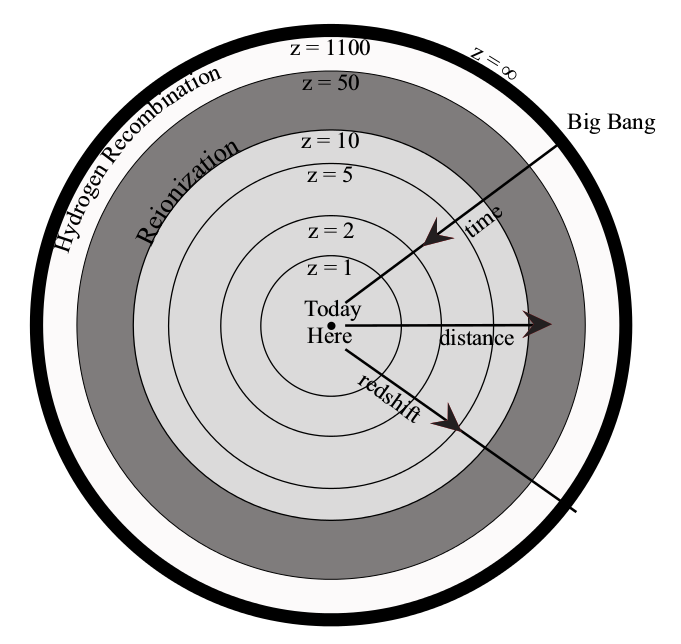
\includegraphics[width=9cm]{MarcoTeorico/historia}
	\caption[Diagrama de tiempo del universo]{Diagrama de tiempo del universo\footnotemark}
	\label{fig:red}
\end{figure}
\footnotetext{Imagen tomada de \cite{loeb}}

Pero la constante de Hubble puede cambiar con el avance del tiempo, de manera que como las demás constantes se define un valor actual y su avance hacia atrás en el tiempo. Por ejemplo, volviendo a la ecuación \ref{eq:En}, se asume que en el presente $\Omega_0=1=(\Omega_\Lambda+\Omega_m+\Omega_r)$, para lo cual la primera contribución corresponde a la densidad de energía del vacío (Energía Oscura), el segundo término corresponde a la materia (tanto oscura como ordinaria o bariónica ($\Omega_b$) y la contribución energética de la radiación. Estos parámetros de distribución de energía son las semillas que pueden llevar a diferentes universos y son precisamente los parámetros de entrada para las simulaciones realizadas en este proyecto. La expresión general para los parámetros está dada por la Ecuación (\ref{eq:total}).

\begin{equation}
\frac{H(t)}{H_0}=\left[\frac{\Omega_m}{a^3}+\Omega_\Lambda+\frac{\Omega_r}{a^4}\right]^{\frac{1}{2}}
\label{eq:total}
\end{equation}


\subsection{Formación de estructura y halos de materia oscura}
Para describir el origen de la Ecuación (\ref{eq:total}) y la dinámica del universo en general, se vuelve necesario introducir una serie de variables que puedan llevar cuenta de los cambios existentes en él. Las primeras son conocidas como las coordenadas comóviles, las cuales a diferencia de las coordenadas fijas tienen en cuenta el factor de expansión del universo $a(t)$, de manera que todo vector de posición $\vec{r}$ tiene asociado unas coordenadas comóviles $\vec{x}=\vec{r}/a$. Por otro lado, al describir cualquier magnitud vectorial es necesario introducir un marco de referencia; por ejemplo, en la tierra el marco de referencia estático es el planeta en sí mismo y el movimiento de los objetos es referido respecto al suelo. Pero cuando comenzamos a trabajar en un panorama más amplio, como lo son las grandes secciones del universo, y donde el vacío domina impidiendo dar una referencia clara, es importante introducir lo que se conoce como las velocidades peculiares. Al caracterizar el movimiento y distancia de estrellas y galaxias lejanas, la velocidad peculiar es aquella componente de velocidad que no se explica a través de la Ley de Hubble de la Ecuación (\ref{eq:hub}), y viene siendo la velocidad del marco de reposo local, dada por la Ecuación (\ref{eq:peculiar}).

\begin{equation}
\vec{u}=\vec{v}-H\vec{r}
\label{eq:peculiar}
\end{equation}

Paralelo a esto, se modela la expansión cosmológica como un fluido ideal, sin presión y en expansión. Además, definen las fluctuaciones fraccionales de densidad como se muestra en la Ecuación (\ref{eq:delta}), en donde $\bar{\rho}$ corresponde a la densidad de masa promedio. Finalmente se define el potencial gravitacional a través de la ecuación de Possion para la gravitación Newtoniana, mostrada en la Ecuación (\ref{eq:poisson}).

\begin{equation}
\delta(\vec{x})=\frac{\rho(\vec{r})}{\bar{\rho}}-1
\label{eq:delta}
\end{equation}


\begin{equation}
\nabla^{2}\phi=4\pi G\bar{\rho}a^{2}\delta
\label{eq:poisson}
\end{equation}


Estas definiciones se realizan para plantear la ecuación de continuidad y la Ecuación de Euler que permiten describir el fluido así:

\begin{align}
\frac{\partial\delta}{\partial t}+\frac{1}{a}\nabla\cdot[(1+\delta)\vec{u}]&=0 \\
\frac{\partial\vec{u}}{\partial t}+H\vec{u}+\frac{1}{a}(\vec{u}\cdot\nabla)\vec{u}&=-\frac{1}{a}\nabla\phi
\end{align}

Todas las ecuaciones mostradas anteriormente dan como resultado la ecuación diferencial mostrada en (\ref{eq:diff}). Hay que tener en cuenta que el comportamiento del fluido estará bien definido para la evolución de partículas de materia oscura sin colisión siempre y cuando no se crucen. Pero los cruces se darán una vez crezcan las perturbaciones y la relación sea no linear con $|\delta|>1$. La Ecuación (\ref{eq:diff}) Tiene dos soluciones, de las cuales sólo una es creciente, y es proporcional a $D(t)$, el cual es llamado el factor lineal de crecimiento \cite{knobel}. En épocas tempranas del universo cuando dominaba la materia ($1<z<10^{3}$) tenemos un factor de crecimiento tal que $D(t) \propto t^{\frac{2}{3}}\propto a(t)$, pero a medida que avanzamos, los crecimientos son cada vez más lentos, al punto que después de la época inflacionaria, cuando el universo es dominado por la Constate de Hubble, todas las fluctuaciones en el campo de densidades quedan congeladas. Lo que esto quiere decir es que por más que existan lugares en el universo en el que se generan condiciones cerradas que colapsan en sí mismas, i.e. galaxias, el potencial gravitacional permanece intacto en magnitud, y por ello las fluctuaciones que observamos en el potencial gravitacional que observamos hoy en día son del mismo orden de magnitud que las que se observan en el CMB.

\begin{equation}
\frac{\partial^{2}\delta}{\partial t^{2}}+2H\frac{\partial\delta}{\partial t}=4\pi G\bar{\rho}\delta
\label{eq:diff}
\end{equation}

Cuando una sobredensidad comienza a atrapar material y entra en la zona de crecimiento no lineal, esta zona frena su expansión, hay un punto de retorno y finalmente colapsa. Estas regiones son conocidas como \textit{halos} de materia oscura, y allí es donde la materia ordinaria se combina para generar nuevos cuerpos. Es por eso que toda galaxia está rodeada o inmersa en un halo de materia oscura, lo explica la velocidad de rotación tal que sigue existiendo un estado ligado (si ni hubiera presencia de la materia oscura, la velocidad de rotación sería superior a la velocidad de escape) para las estrellas y sistemas formados. Así que si se modela las regiones de sobredensidad como una región esférica cuya función de densidad cumple con un perfil cuadrado (``sombrero de copa''), se pueden resolver analíticamente las ecuaciones de evolución llegando a que una región esférica dejará de expandirse para colapsar a un punto, si su sobredensidad en un tiempo $z$ está dada por,

\begin{equation}
\delta_{crit}(z)=\frac{1.686}{D(z)}
\label{eq:critdens}
\end{equation}


\section{Simulación en Paralelo y Análisis}
Como se dijo en la Sección \ref{sec:universo}, la materia oscura tiene las mismas propiedades gravitatorias que la materia ordinaria u observable, pero la supera en cantidad por casi 5 veces en todo el universo. Es por esto que para analizar las estructuras a gran escala el universo, la distribución de materia, los grandes halos y la dinámica de la materia en el universo se puede partir del análisis de materia oscura, puesto que se espera que la materia ordinaria esté ubicada en donde existan mayores concentraciones de materia oscura. Si bien no tenemos forma de observar los cambios en el universo si se cambia la distribución de energías, se pueden realizar simulaciones a gran escala de todo el universo variando los parámetros cosmológicos. En la siguiente sección se explicará brevemente las características de los algoritmos utilizados y su modo de funcionamiento.


\subsection{Gadget-2 y N-GenIC}

Toda simulación de un entorno estará limitada por el recursos computacionales que se tengan, como por ejemplo el tiempo de simulación, la cantidad de procesadores disponibles y la cantidad de memoria que se puede ocupar. De manera que la eficiencia de un código estará dictada por la eficiencia en consumo de dichos recursos; qué tantos recursos consume y qué tan exactos son los resultados obtenidos. Existe una gran variedad de códigos para la simulación de $N$ partículas con diversas ventajas y desventajas entre cada uno, pero la principal diferencia radica en el método de análisis de cada código para realizar aproximaciones a pequeña y gran escala, permitiendo así una cierta tolerancia sin comprometer mayor cantidad de recursos. Gadget-2 es un código creado por Volker Springel y publicado en el 2005\cite{gadget} para realizar grandes simulaciones cosmológicas de $N$ cuerpos. La principal ventaja de este código es la efectividad en el manejo de gran y pequeña escala, pues dentro de un cierto rango, realiza cálculos detallados de la gravedad, pero para mayores distancias realiza un análisis de Fourier que calcula la gravedad efectiva aproximada.

La primera característica del código de Gadget-2 es la creación de un \textit{octree} BH para el análisis de las partículas, lo cual significa que se crea un árbol de análisis en el cual cada nodo puede tener 8 hojas o ramificaciones. Este algoritmo permite que la fuerza gravitacional computacional calculada para cada partícula sea realizada por $\mathcal{O}(\log N)$ interacciones, contrario a los algoritmos de suma directa los cuales necesitan $\mathcal{O}(n^{2})$ interacciones. Para la generación del \textit{octree} se parte del cubo inicial, el cual se divide en 8 octantes iguales y luego se decide si cada subdivisión debe partirse nuevamente en 8 partes hasta que cada partición realizada (hoja del árbol) tiene 1 o 0 partículas en ella, comos se puede observar en la Figura \ref{fig:octree}. 

\begin{figure}[H]
	\centering
	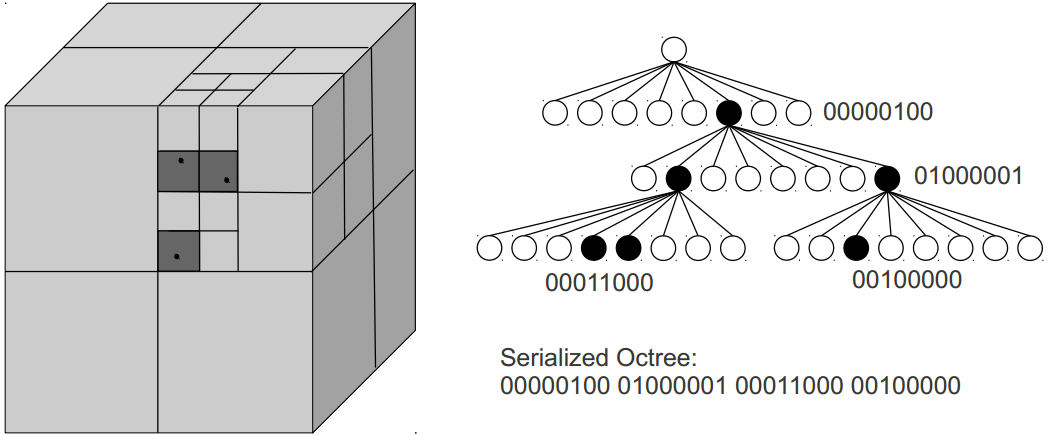
\includegraphics[width=0.7\textwidth]{MarcoTeorico/octree_encode}
	\caption[División del espacio con octree]{División del espacio con octree \footnotemark}
	\label{fig:octree}
\end{figure}
\footnotetext{Imagen tomada de \url{http://traumabot.blogspot.com/2013/06/octree-based-point-cloud-stream.html}} 

De esta manera, al tener construido el árbol, sólo resta recorrerlo para calcular las fuerzas efectivas. Así que se inicia por la raíz del árbol o el nodo principal y de acuerdo a las características del nodo, se decide se explorar más allá o no, y en dado caso recorrer las 8 ramificaciones para la contribución de la fuerza efectiva. En el caso de que un nodo esté lo suficientemente lejos, toda la sección del árbol que se encuentra de allí en adelante se considera como la contribución de un único cuerpo. Finalmente para la efectividad del código y la compatibilidad con el SPH (\textit{Smoothed particle hidrodynamics}) no se realizan expansiones multipolo del momento sino que se usa el monopolo de momento. 

\begin{equation}
\phi(x)=\sum\limits_i m_i\varphi(x-x_i)\xrightarrow{\mathscr{F}}\phi^{short}_{k}+\phi^{long}_{k}
\label{eq:phifourier}
\end{equation}

La Ecuación (\ref{eq:phifourier}) muestra el análisis que se debe realizar para el potencial peculiar gravitacional por Gadget-2, pero además de esto, se realiza una descomposición en el espacio de Fourier para discernir entre los efectos lejanos y cercanos. Para la parte real es suficiente realizar un análisis en el espacio real mediante la función de error complementario, como se muestra en la Ecuación (\ref{eq:erfc}), en donde $r_i=min(|\vec{x}-\vec{ri}-nL|)$, ya que la función de error complementario rápidamente suprime cualquier contribución distante. Por otro lado, para las contribuciones lejanas del potencial se vuelve mucho más sencillo realizar un análisis mediante métodos de mallados en espacio de Fourier. Este proceso, en conjunto con el método Tree, se le llama frecuentemente como el \textit{TreePM Method}.

\begin{equation}
\phi^{short}_k(x)=-G\sum\limits_i\frac{m_i}{r_i}erfc\left(\frac{r_i}{2r_s}\right)
\label{eq:erfc}
\end{equation}





%Metodología
\chapter{Metodología del Trabajo}
\label{chap:metodologia}
El desarrollo de este proyecto se basó en una metodología completamente computacional, debido a que el trabajo principal fue la realización de múltiples simulaciones y la creación e implementación de códigos y programas para su análisis. La metodología propuesta y usada a lo largo del semestre se puede resumir en la Figura \ref{fig:meto} en donde se pueden ver las diferentes etapas del proyecto. En la primera etapa se consultó el material bibliográfico disponible tanto para la generación de simulaciones a través de Gadget-2 \cite{gadget}, así como para la comprensión de los conocimientos básicos para el desarrollo del proyecto, explicados en el Capítulo \ref{chap:marco}. 

\begin{figure}[H]
	\centering
	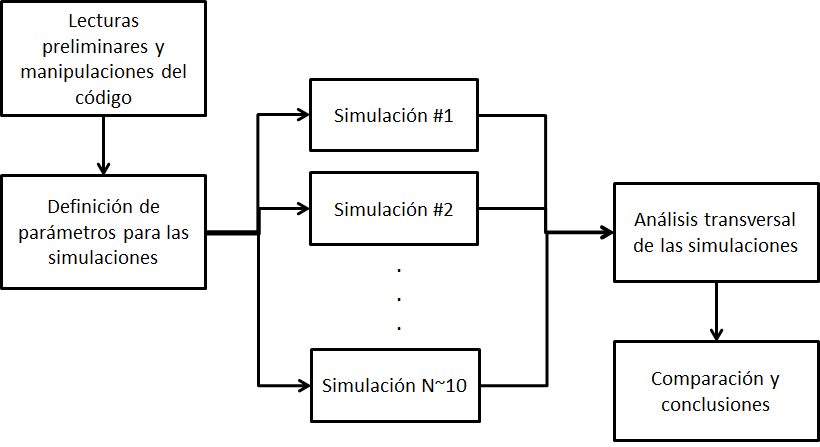
\includegraphics[width=11cm]{Metodologia/metodologia.png}
	\caption{Metodología de trabajo}
	\label{fig:meto}
\end{figure}

Una vez instaladas todas las librerías y códigos necesarios en el cluster de física, se procedió a realizar una serie de simulaciones preliminares. Éstas tenían como objetivo principal observar la dinámica del código, sus posibles errores, medir el tiempo de computación y sobretodo tener una muestra de los archivos exportados en cada simulación para poder analizarlos, ver su estructura y la información que contenían y en base a ello comenzar a escribir códigos de análisis que servirían para las simulaciones grandes. Estas primeras simulaciones se basaban en cajas cúbicas periódicas de lado de $150Mpc$ y contenían $128^3$ y $256^3$ partículas.

Una vez realizadas todas las pruebas preliminares se prepararon las condiciones iniciales para las simulaciones definitivas, las cuales por restricción de tiempo y recursos computacionales se fijaron a un cubo de $500Mpc$ de lado con un total de $512^3$ partículas. Dado el número de partículas, el tiempo de simulación comenzó a aumentar en un factor de 8, así que mientras que las simulaciones de $128^3$ partículas tomaban alrededor de 3 horas, las siguientes tomaron un día entero. Desafortunadamente al momento de correr las simulaciones definitivas, estas no fallaron por falta de memoria en el cluster de la universidad, por más que se corrieran en los 56 procesadores no lograba tener registro de todas las partículas. 

\textcolor{red}{Se corrieron las simulaciones en el cluster de Corea y...}

El análisis realizado a los resultados de las simulaciones tuvo dos vertientes principales: análisis por halos de materia oscura y análisis de fluctuaciones de densidades. De igual manera se generaron dos secuencias de código independientes para cumplir con ambos propósitos. Para la primera se hizo uso de un código existente para la búsqueda de halos por medio del algoritmo FoF y posteriormente se usó la información de los halos, como por ejemplo sus centros de masa y velocidades respectivas, tanto para un análisis intrínseco de cada simulación como para un análisis transversal entre las simulaciones \textcolor{red}{completar}. Para la segunda vertiente se calculó el campo de densidades de cada una de las simulaciones para realizar un análisis del espectro de fluctuaciones en cada caso. Para cada una de las simulaciones finales se varió la proporción de materia y energía oscura en el universo.

\section{Cronograma de Trabajo}
A continuación, en la Tabla \ref{tab:crono} se muestra el plan de trabajo propuesto para la realización del proyecto, junto con la distribución de tiempo establecida para la realización de cada una de las tareas.

\begin{table}[H]
	\centering
	\begin{tabular}{>{\centering}p{5cm}cp{7.5cm}}
		\hline \hline
		\textbf{Actividad} & \textbf{Duración} & \textbf{Descripción} \\
		\hline
		Lectura de Bases teóricas & 2 semanas & Revisión bibliográfica acerca de la composición del universo y los parámetros que definen su evolución.\\
		Lectura e instalación del código & 2 semanas & Instalación de librerías y entornos necesarios. Familiarización con los métodos de simulación y los códigos y lenguajes a usar.\\
		Simulaciones preliminares & 3 semanas & Realización de simulaciones de bajo nivel, observando archivos exportados y comportamiento.\\
		Simulaciones definitivas & 4 semanas & Adquisición de datos definitivos de análisis con simulaciones de alto nivel computacional.\\
		Análisis de simulaciones y creación de códigos& 3 semanas & Creación de programas de análisis en base a los formatos de exportación de Gadget-2 y generación de estadísticas y comparaciones.\\
		Redacción de documento & 3 semanas & Recoger los datos obtenidos y resultados de los análisis para redactar documento final.\\		
		\hline
	\end{tabular}
	\caption[Cronograma de Trabajo]{Cronograma de Trabajo \footnotemark}
	\label{tab:crono}
\end{table}

\footnotetext{La realización de las tareas no fue secuencial y los tiempos mostrados se sobrelapan durante el semestre}





%Trabajo realizado
\chapter{Trabajo Realizado}
\label{chap:trabajo}

\section{Características de Simulación}
El trabajo realizado a lo largo del semestre se puede dividir en dos secciones principales: la realización de simulaciones y la escritura de códigos de análisis y comparación para dichas simulaciones. Para el primer caso implica la lectura de cómo correr las simulaciones en clusters de múltiples procesadores, definir los parámetros de instalación y de simulación en sí y observar los comportamientos, tiempos de duración y modos de exportación de datos de cada simulación. Para la segunda sección se incluyen los códigos realizados y utilizados que permiten desde la lectura de los datos brutos de simulación hasta la extracción de propiedades y generación de gráficas de análisis. A continuación se explicarán las diferentes secciones y detalles del trabajo realizado, así como los resultados de dicho trabajo.

\subsection{Parámetros de instalación y compilación}
Para correr una simulación en Gadget-2 se requiere principalmente de 3 librerías previamente instaladas y de un set de condiciones iniciales sobre las cuales trabajar. Las tres librerías que se deben instalar son FFTW, GSL y MPI, todas ellas de libre distribución e instalación. FFTW es una librería, o conjunto de librerías, con códigos para la realización de transformadas de Fourier en espacio discreto, como la transformada rápida de Fourier (FFT), cuyo uso se explicó en la Sección \ref{sub:gadget}. GSL (\textit{GNU Scientific Library}) como su nombre lo dice es una librería con un gran conjunto de funciones de uso científico. Finalmente, MPI (\textit{Message Passing Interface}) es la librería de instrucciones, rutinas y métodos para la paralelización de procesos en múltiples procesadores. 

Como se explicará más a fondo en la Sección \ref{sub:simulaciones}, las simulaciones fueron realizadas no sólo en computadores personales sino que también se hizo uso del clúster de física de la Universidad de los Andes y además del clúster KIAS en Corea 
\subsection{Parámetros de la simulación}

\subsection{Simulaciones realizadas}
\label{sub:simulaciones}


\section{Códigos de Análisis}

\subsection{Estructura del \textit{Snapshot}}

\subsection{Extracción de Halos}



\subsection{Campo de densidades (CIC)}
\label{sub:CIC}

\section{Análisis y Resultados}


%Validación de los resultados
%\input{Validacion/validacion.tex}

%\input{discusion.tex}

\chapter{Conclusiones}
En conclusión se observó que en caso de querer realizar análisis estadísticos para observaciones en el universo en pro de querer realizar medidas de los parámetros cosmológicos, una análisis mediante mediciones de redshift, los cambios que deberá detectar son del orden de $\frac{\Delta v}{c}=700/300000\approx 2\times10^{-3}$, algo que es alcanzable solamente con los experimentos de próxima generación, entre ellos DESI. 


Además de esto, encontramos que un análisis mediante mediciones de masas sería inviable ya que los cambios de masa que caerían en variaciones de $5\%$ en $\Omega_0$ son cercanos a un factor de 2. Esto es indetectable con los métodos actuales, ya que los factores más bajos detectables con la tecnología disponible son cercanos a 10.


\section{Trabajo Futuro}
\begin{enumerate}
	\item Tomar los resultados de las simulaciones resultado del proyecto para la realización de observaciones virtuales para cuantificar los efectos del \textit{redshift space distorsion} en observaciones.
	\item Cuantificar en detalle la influencia de la red cósmica en la formación y alineación de halos de materia oscura con la estructura a gran escala.
	\item Utilizar los resultados de las simulaciones como laboratorio de estudio de formación y evolución de poblaciones de galaxias observables con experimentos de siguiente generación, como DESI o HETDEX.
\end{enumerate}


%Bibliografia
\phantomsection % To make hyperref link in TOC work correctly
\addcontentsline{toc}{chapter}{\bibname} % puts entry
\nocite{*}
\bibliographystyle{abbrv}
\bibliography{references}

%Apéndices
\appendix

%Cambio de estilo para nombres de los capítulos en Apéndices
\titleformat{\chapter}[display]% display permite un cambio de línea entre el número y el título
   {\normalfont\huge\bfseries}{\raggedright\chaptertitlename\ \thechapter}{1em}{\Huge}

%Resumen ejecutivo
%\input{Ap_ResumenEjecutivo/resumenEjecutivo.tex}

%Datos EDX
%\input{Ap_DatosEDS/datosEDS.tex}


\end{document}